\title{Subsets and Subspaces}
\subtitle{\SubTitleName}
\institute[]{\Course}
\author{\Instructor}
\maketitle  



\frame{\frametitle{Topics and Objectives}
\Emph{Topics} \\
\TopicStatement
\begin{itemize}
    \item subsets and subspaces
    \item set builder notation
\end{itemize}

\vspace{0.5cm}

\Emph{Objectives}\\

\LearningObjectiveStatement

\begin{itemize}
    \item determine whether a subset of $\mathbb R^n$ is a subspace
    % \item determine whether a vector is in a particular subspace, or find a vector in that subspace
    % \item construct a basis for a subspace (for example, a basis for Col(A))
\end{itemize}


}


\frame{\frametitle{Subsets of $\mathbb R^n$}

    
    \begin{center}\begin{tikzpicture} \node [mybox](box){\begin{minipage}{0.80\textwidth}\vspace{2pt}

        A \Emph{subset of $\mathbb R^n$} is any collection of vectors that are in $\mathbb R^n$.
        
    \end{minipage}};\node[fancytitle, right=10pt] at (box.north west) {Definition};
    \end{tikzpicture}\end{center}
    
    \Emph{Examples}
    \begin{itemize}
        \item the span of the columns of a $3\times4$ matrix is a subset of $\mathbb R^3$
        \item the set of all vectors of the form $\spalignmat{1;k}$ is a subset of  $\mathbb R^2$
    \end{itemize}
    
}

\frame{\frametitle{Subspaces in $\mathbb R^n$}

    % ~~ ~~ Highlight Box ~~ ~~
    \begin{center}\begin{tikzpicture} \node [mybox](box){\begin{minipage}{0.90\textwidth}\vspace{2pt}

    A subset $ H $ of $ \mathbb R ^{n}$ is a \Emph{subspace} if it is closed under scalar multiplies and vector addition.  That is: for any $c\in\mathbb R$ and for $\vec u,  \vec v\in H$, 

    \begin{enumerate}
        \item $c \,\vec u  \in H$
        \item $\vec u + \vec v \in H$
    \end{enumerate}
    \end{minipage}};\node[fancytitle, right=10pt] at (box.north west) {Definition};
    \end{tikzpicture}\end{center}

    Note that condition 1 implies that the zero vector must be in $H$.

}



\frame{\frametitle{Example: Subspaces}
    Which of the following subsets could be a subspace of $\R^2$? 

    \begin{center}
    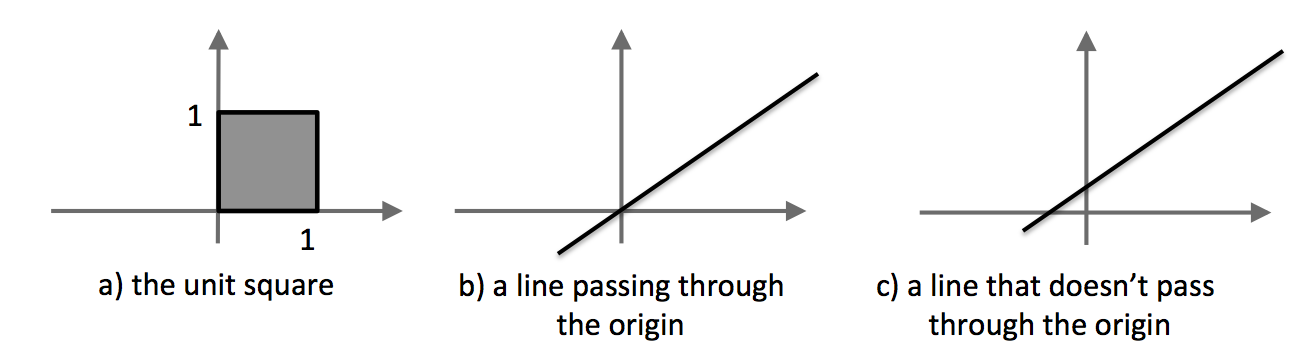
\includegraphics[width=0.95\textwidth]{Chapter2/images/subspaces.png} 
    \end{center}

}

\frame{\frametitle{Example: Set Builder Notation}

    Let $V = \left\{ \spalignmat{a ; b} \in \mathbb R^2 \ | \ ab = 0 \right\}$. 
    \begin{enumerate} 
        \item Give an example of at least two vectors that are in $V$. 
        \item Give an example of at least two vectors that are not in $V$. 
        \item Is the zero vector in $V$? 
        \item Is $V$ a subspace? 
    \end{enumerate}

}




\frame{\frametitle{Summary}

    \SummaryLine \vspace{4pt}
    \begin{itemize}\setlength{\itemsep}{8pt}
        \item identifying whether a subset is a subspace
    \end{itemize}
    

}